\documentclass{beamer}
%\documentclass[aspectratio=169]{beamer}
\mode<all>
{
  \usetheme{default}      % or try Darmstadt, Madrid, Warsaw, ...
  \usecolortheme{default} % or try albatross, beaver, crane, ...
  \usefonttheme{default}  % or try serif, structurebold, ...
  \setbeamertemplate{navigation symbols}{}
  \setbeamertemplate{caption}[numbered]
  \setbeamertemplate{itemize items}[circle]
  \setbeamertemplate{frametitle}{\textbf{\insertframetitle}\\\small\insertframesubtitle}
  %\setbeamertemplate{frametitle}{\bfseries\insertframetitle\par}
}

\usepackage[english]{babel}
\usepackage[utf8]{inputenc}
%\usepackage[T1]{fontenc}

\usepackage{framed}
\usepackage{amssymb}
\usepackage{amsmath}
\usepackage{amsthm}
\usepackage{graphicx}
\usepackage{makecell}
\usepackage{wrapfig}
\usepackage{float}
\usepackage{booktabs}

\newcommand\Wider[2][3em]{%
\makebox[\linewidth][c]{%
  \begin{minipage}{\dimexpr\textwidth+#1\relax}
  \raggedright#2
  \end{minipage}%
  }%
}


\title{\textbf{FunSearch \& AlphaEvolve}}
\author{
\textbf{
Bartosz Piotrowski
}}
\date{
August 21, 2025\\
The Reasoning Reading Group @ FAIR
}

\begin{document}

\begin{frame}
  \titlepage
\end{frame}

\begin{frame}{Motivation}
Preconditions:
\begin{itemize}
\item A problem of finding optimal heuristic/program.
\item A pre-trained, coding-capable LLM.
\item An automated evaluator returning a scalar score.
\end{itemize}
\pause
The simplest strategy:
\begin{itemize}
\item generating multiple independent samples from the LLM with non-zero
 temperature,
\item evaluating all of them,
\item selecting the best one.
\end{itemize}

\pause
But instead of sampling independently, can we \textbf{incorporate the evaluator
feedback} into subsequent generations?

\end{frame}

\begin{frame}{FunSearch}
Key ingredients:
\begin{itemize}
\item \textit{best-shot} prompting,
\item a growing database of programs,
\item an evolutionary strategy acting on it.
\end{itemize}
\end{frame}

\begin{frame}{FunSearch}
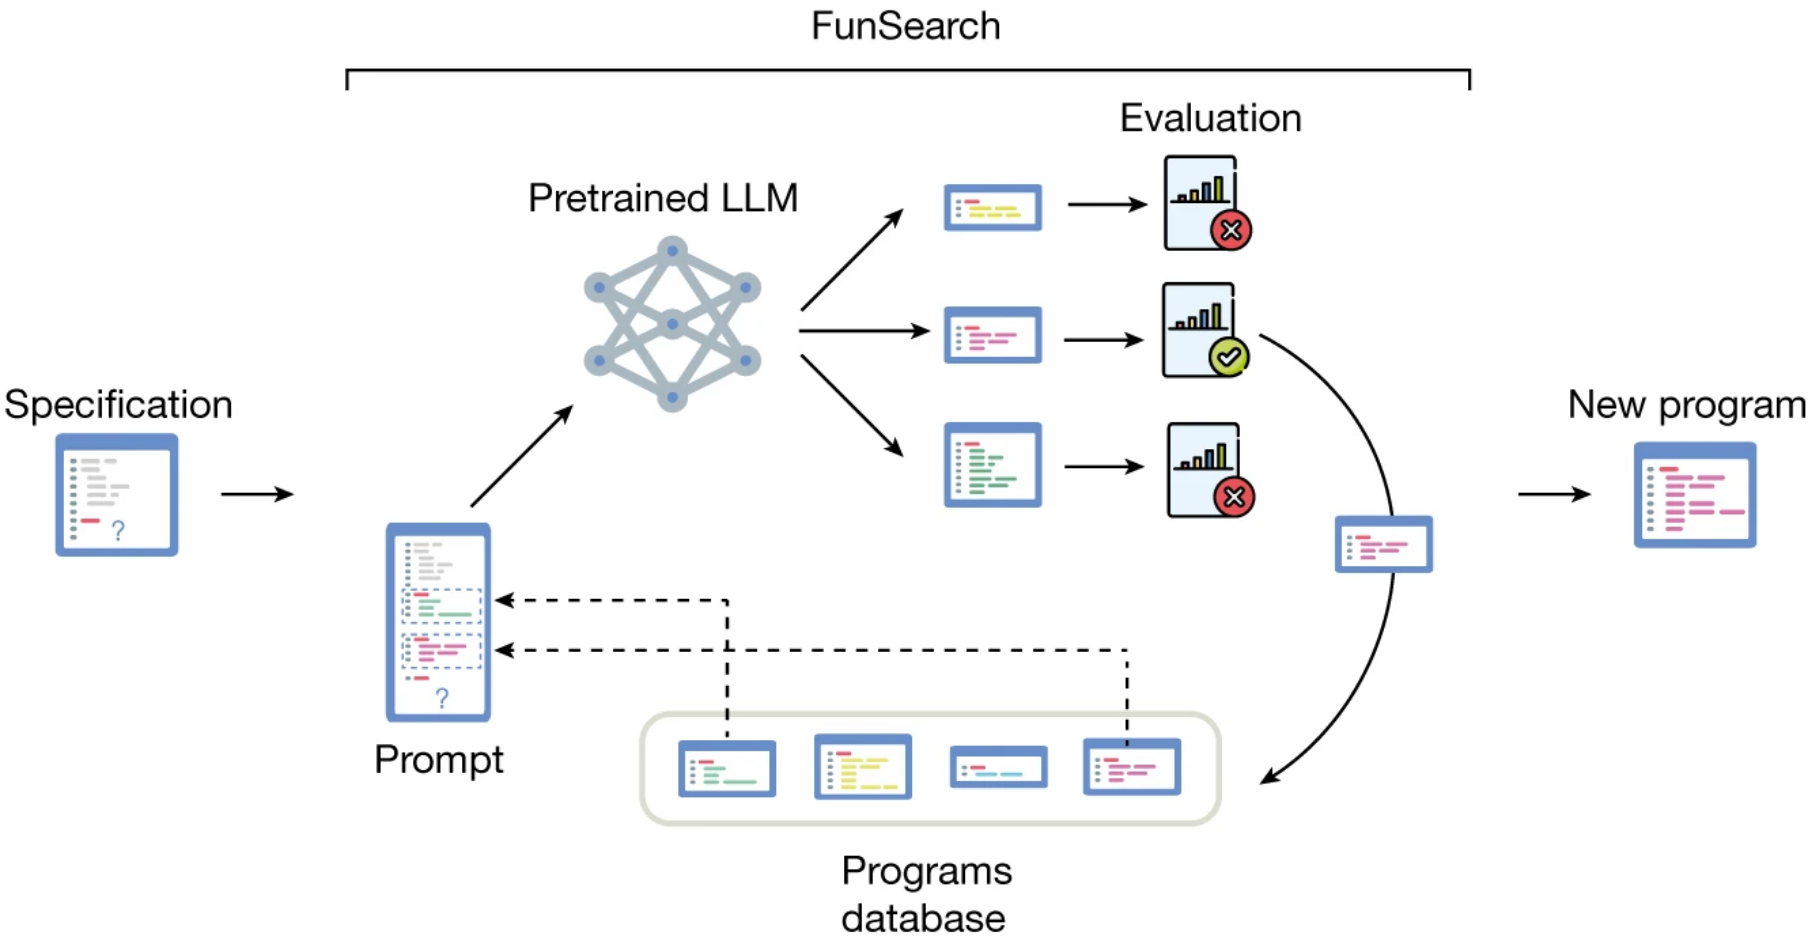
\includegraphics[width=\linewidth]{figures/funsearch-overview.png}
\end{frame}

\begin{frame}{Database of programs}
\begin{itemize}
\item Several island/subpopulations growing independently.
\item Higher-scoring programs, but also shorter ones, are prioritized.
\end{itemize}
\end{frame}

\begin{frame}{Best-shot prompting}
\begin{itemize}
\item $k$ good programs per prompt sampled, for each island.
\item Information which one is better incorporated into the prompt.
\end{itemize}
\end{frame}


\begin{frame}{Cap set problem}
What is the the largest possible set of vectors in $\mathbb{Z}^n_3$
 (\textit{cap set}) such that no three vectors sum to zero?
\pause
\begin{figure}
    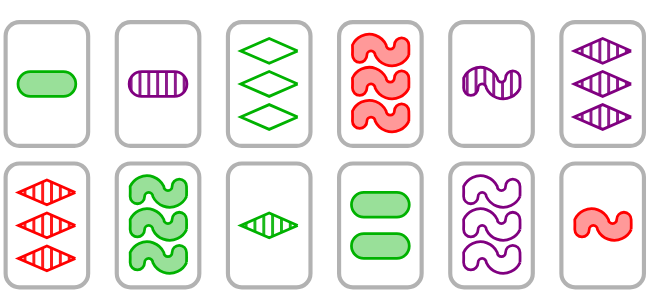
\includegraphics[width=0.6\linewidth]{figures/no-set.png}
\end{figure}
    \pause
\begin{figure}
    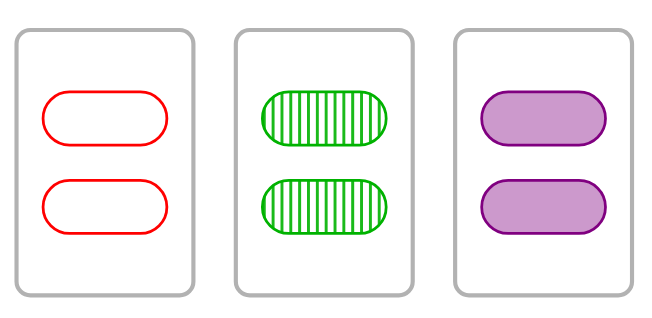
\includegraphics[width=0.4\linewidth]{figures/set.png}
\end{figure}
\pause
\begin{figure}
\centering
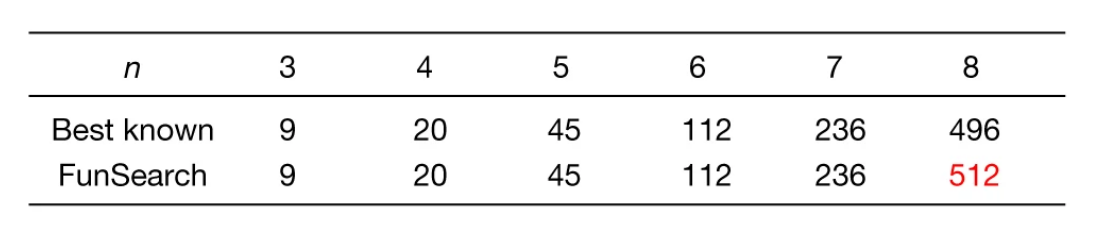
\includegraphics[width=0.7\linewidth]{figures/cup-set-table.png}
\end{figure}
\end{frame}


\begin{frame}{Cap set solution template}
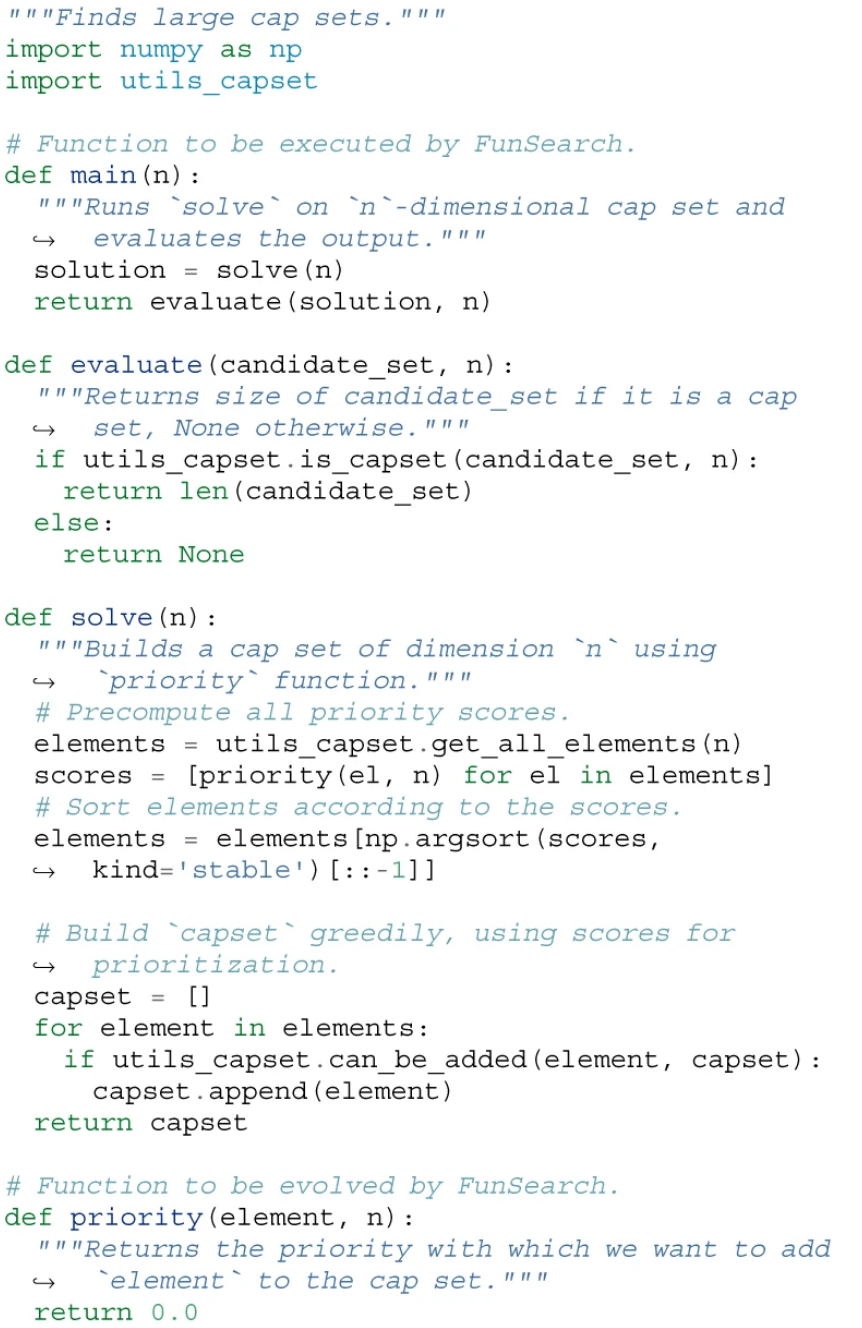
\includegraphics[width=0.5\linewidth]{figures/template.png}
\end{frame}


\begin{frame}{Cap set solution (priority function)}
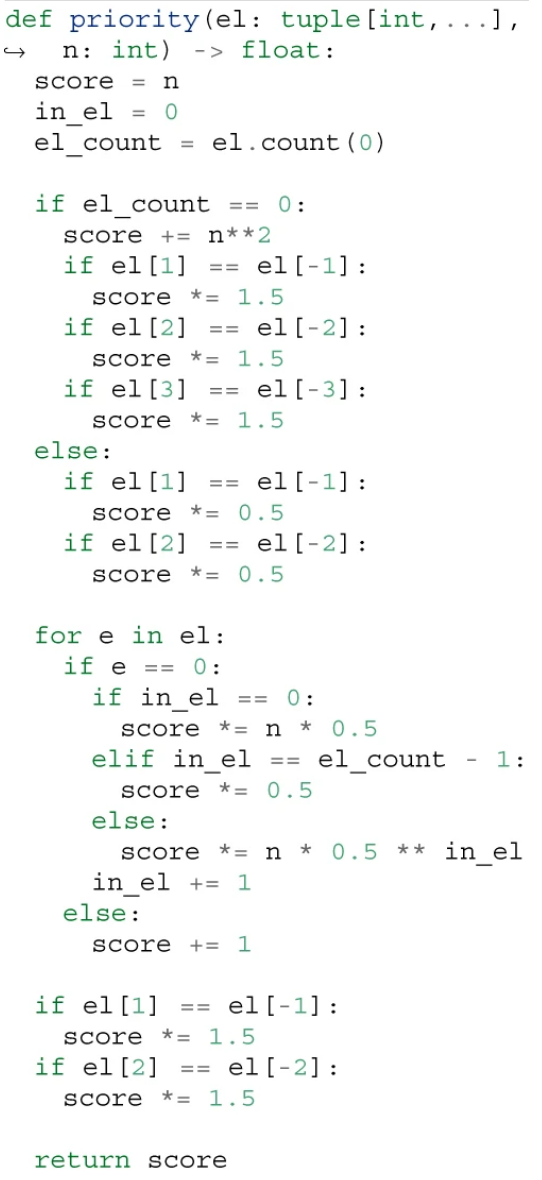
\includegraphics[width=0.5\linewidth]{figures/cup-set-solution.png}
\end{frame}


\begin{frame}{AlphaEvolve}
tldr: FunSearch scaled-up in multiple dimensions. \\
\begin{figure}
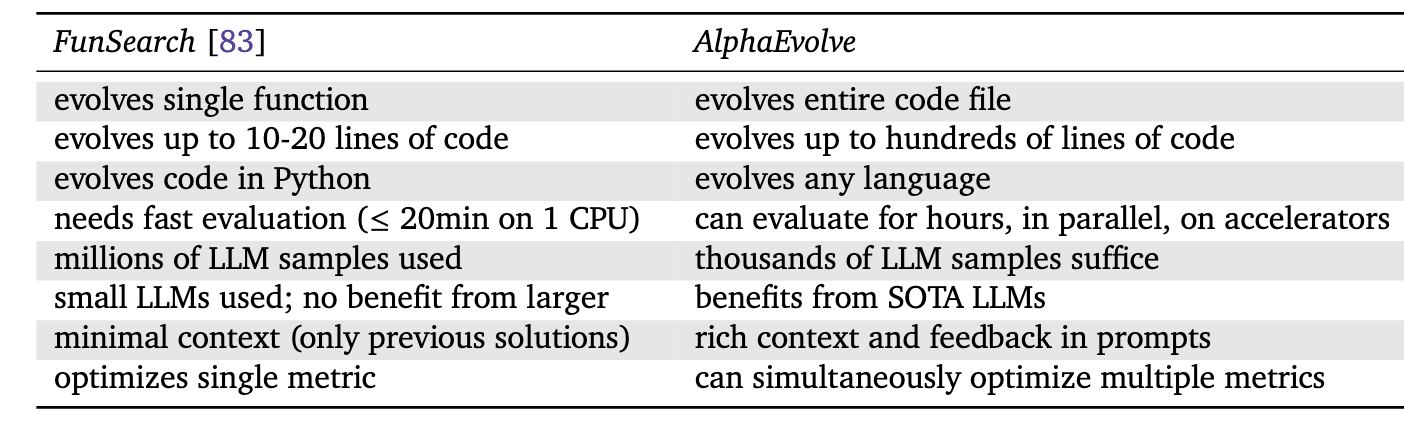
\includegraphics[width=1\linewidth]{figures/funsearch-vs-alphaevolve.png}
\end{figure}
\end{frame}

\begin{frame}{Optimizing matrix multiplications}
\begin{figure}
\centering
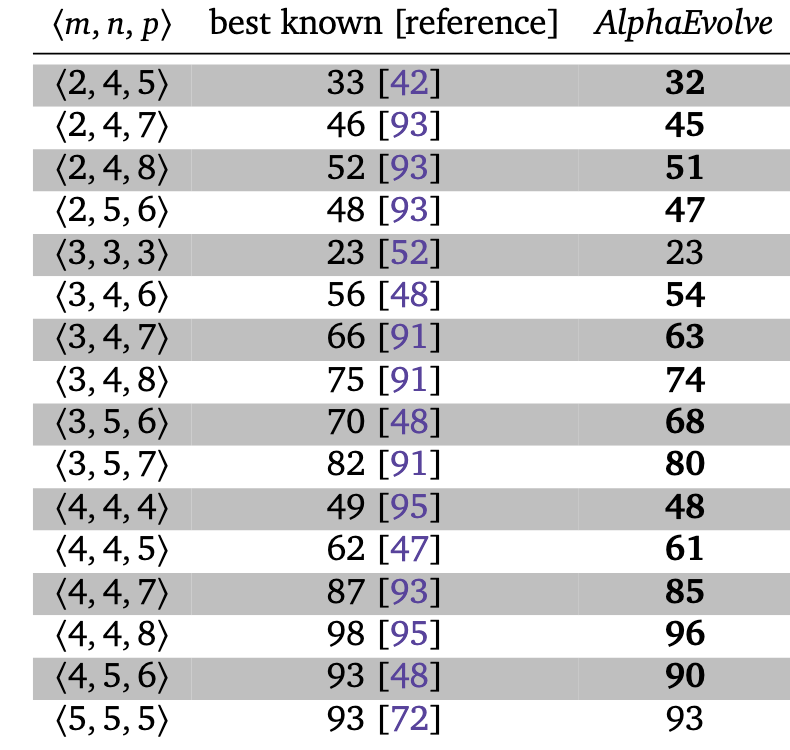
\includegraphics[width=0.5\linewidth]{figures/matmul-table.png}
\end{figure}
\end{frame}

\begin{frame}{Ablations}
\begin{figure}
\centering
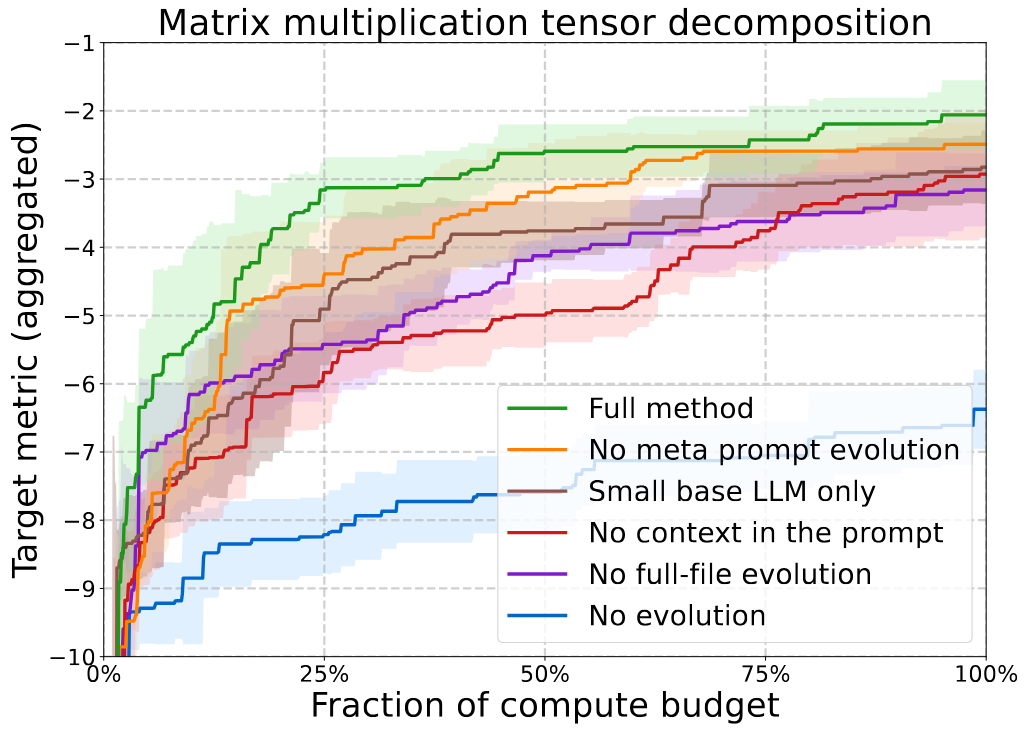
\includegraphics[width=0.8\linewidth]{figures/alphaevolve-ablations.png}
\end{figure}
\end{frame}

\begin{frame}{Closing remarks}
\begin{itemize}
\item
\item
\end{itemize}
\end{frame}


\end{document}
